\documentclass[tikz,border=10pt]{standalone}
\usetikzlibrary{calc,angles,quotes,shapes.geometric}

\begin{document}
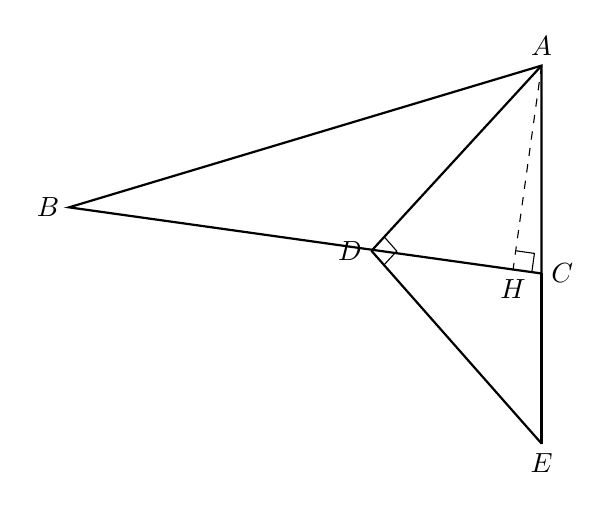
\begin{tikzpicture}[scale=1.2, >=stealth]
    % 1. 定义核心顶点坐标 (基于图像比例估算)
    \coordinate (A) at (4, 3);
    \coordinate (C) at (4, 0.8);
    \coordinate (E) at (4, -1);
    \coordinate (B) at (-1, 1.5);
    
    % 定义 D 点在 BC 连线上
    \coordinate (D) at (2.2, 1.04);
    
    % 计算 H 点：从 A 向直线 BC (即 BD) 作垂线
    % 使用 TikZ 的投影语法标注 H
    \coordinate (H) at ($(B)!(A)!(C)$);

    % 2. 绘制主要实线边界
    \draw[thick] (A) -- (B) -- (C) -- cycle; % 绘制三角形 ABC
    \draw[thick] (A) -- (D);                % 连结 AD
    \draw[thick] (D) -- (E);                % 连结 DE
    \draw[thick] (C) -- (E);                % 连结 CE (AC的延长线)

    % 3. 绘制辅助线 (虚线)
    \draw[dashed] (A) -- (H);               % 高线 AH

    % 4. 标注直角符号
    % 标注 AH \perp BC 处的直角
    \draw ($(H)!0.2cm!(A)$) -- ($(H)!0.2cm!(A) + (H)!0.2cm!(C) - (H)$)- -($(H)!0.2cm!(C)$);
    
    % 标注 AD \perp DE 处的直角 (旋转视角)
    \draw ($(D)!0.2cm!(A)$) -- ($(D)!0.2cm!(A) + (D)!0.2cm!(E) - (D)$)- -($(D)!0.2cm!(E)$);
    
    % 5. 标注文本标签
    \node[above] at (A) {$A$};
    \node[left]  at (B) {$B$};
    \node[right] at (C) {$C$};
    \node[left]  at (D) {$D$};
    \node[below] at (E) {$E$};
    \node[below] at (H) {$H$};

\end{tikzpicture}
\end{document}